\section{Egyszerű DNN model felépítése}
\label{dnn_model}
A továbbiakban egy DNN model alkalmazása olvasható. A megismert cimkéket továbbiakkal egészítettük ki, majd ez alapján generáltunk gerjesztési és spektrális paramétereket, amikből előállítható az audio.

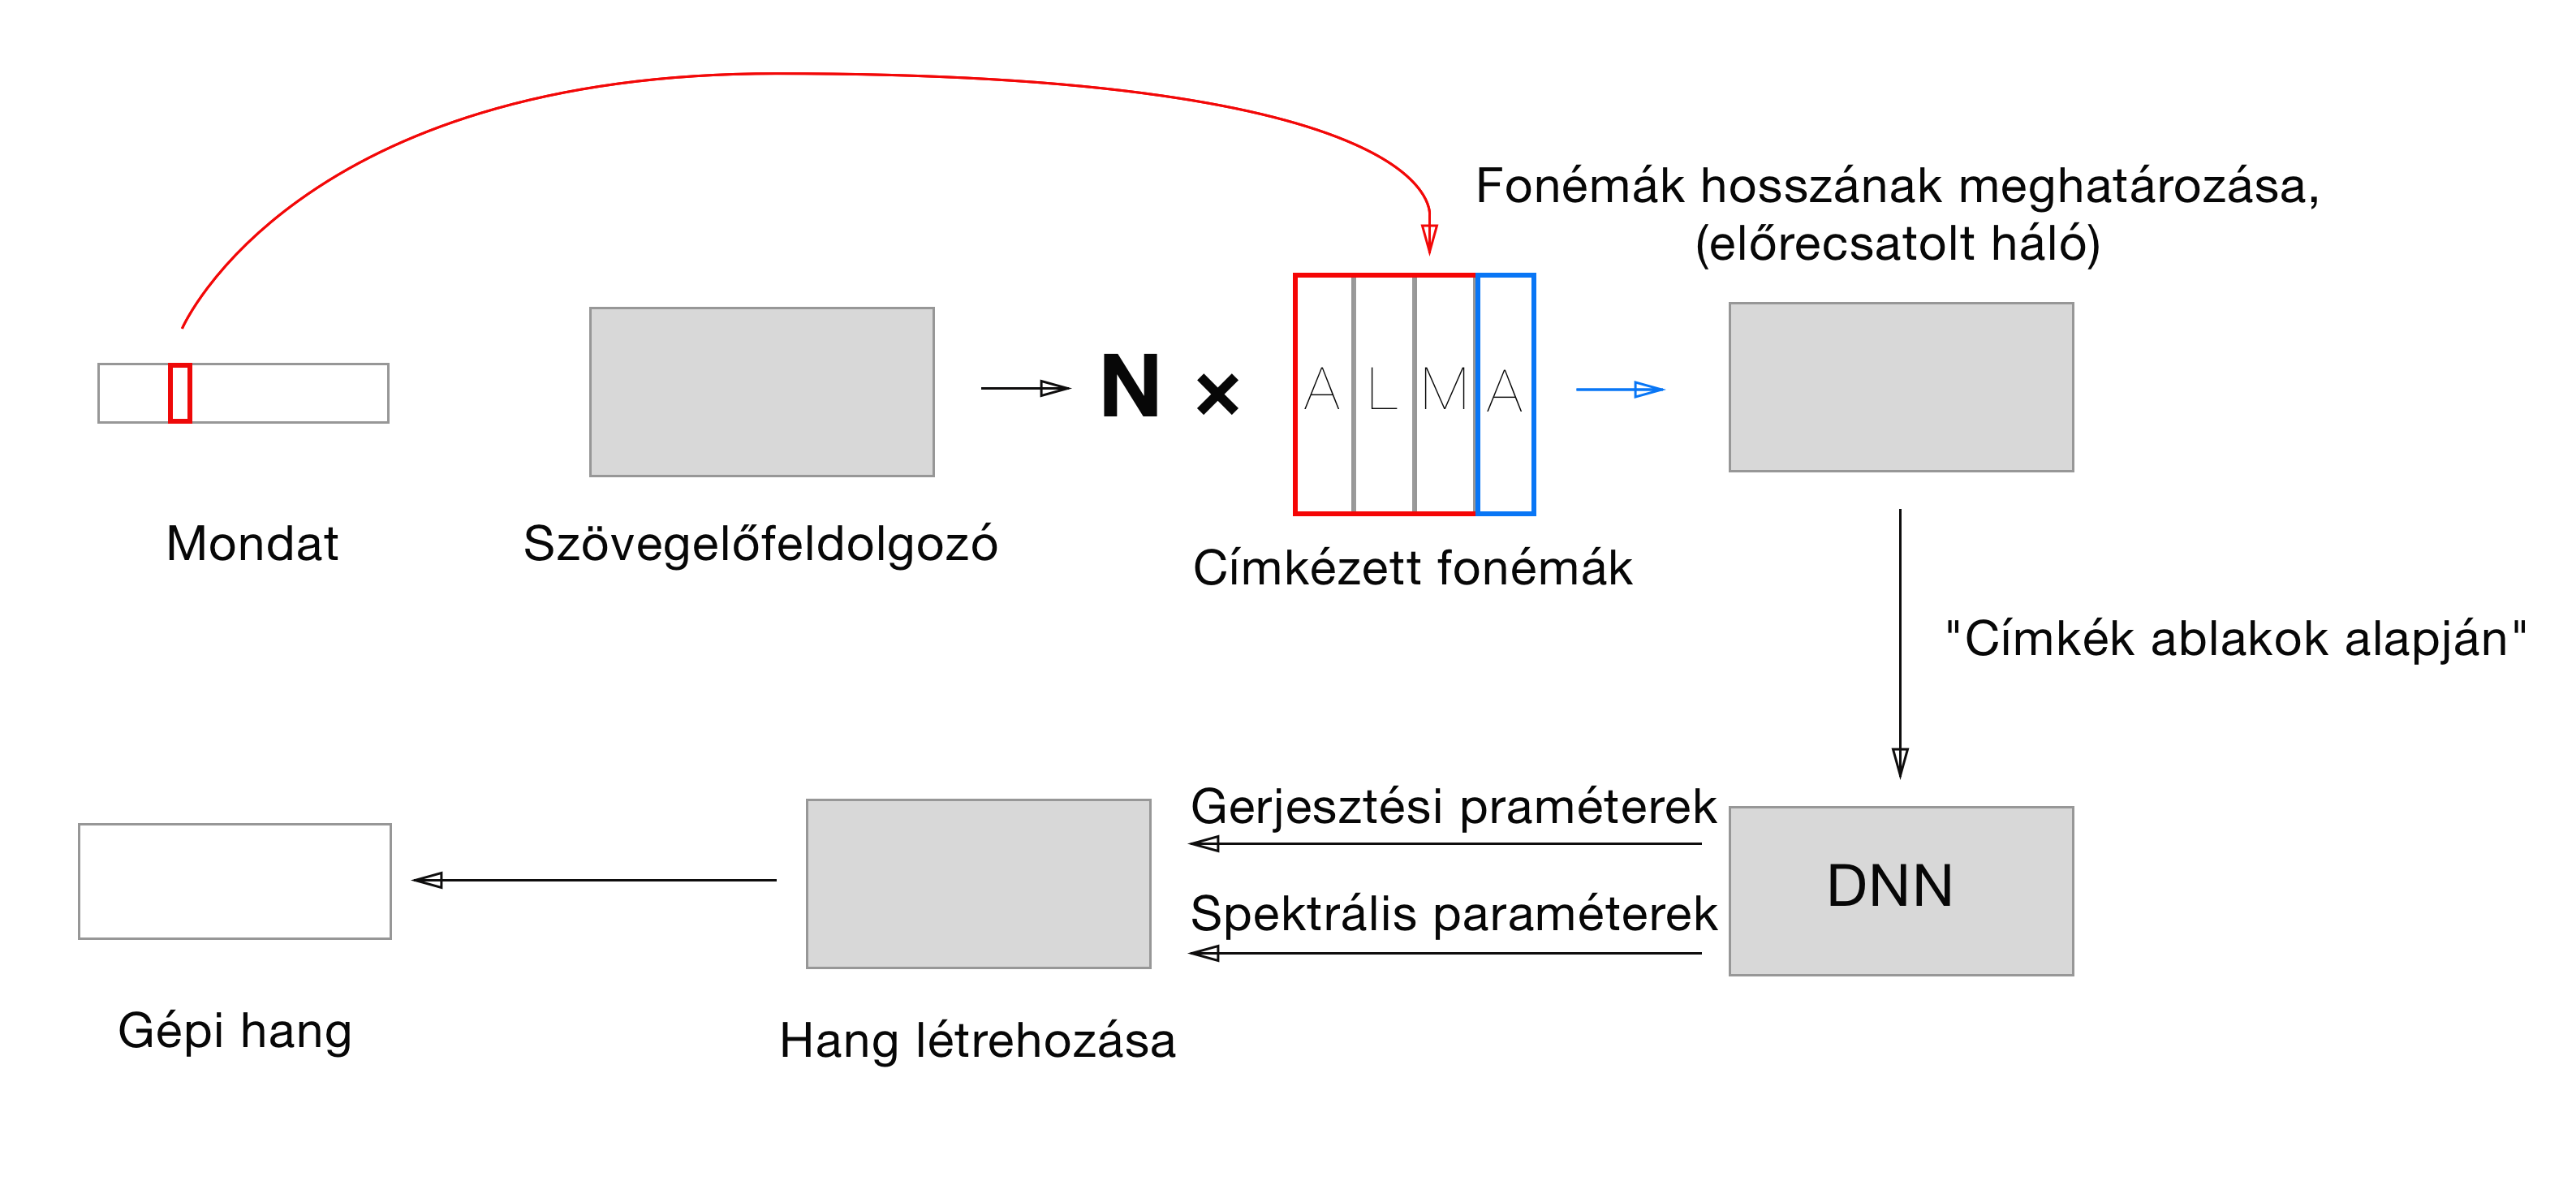
\includegraphics[width=\textwidth,keepaspectratio]{dnn_struct}

\subsection{Háló modell}
Külön hálón tanítottuk a spektrális és a gerjesztési paramétereket. 

Előrecsatolt mély neurális hálózatot építettünk fel, 6 rejtett réteggel, tanh és sigmoid aktivációs függvényekkel, SGD optimalizálóval és MSE költségfüggvénnyel. A háló rétegeire Dropoutot is használtunk. (/!TODO ref)
A megállást early stoppinggal detektáltuk.

/!TODO háló modell kép